% Note: remove `openany` for printed version
\documentclass[12pt,a4paper,openany,dutch,english]{extbook}
\usepackage[a4paper,includeheadfoot,margin=2.50cm]{geometry}


% By default, LaTeX tries to stretch whitespace between paragraphs on a page in order to reduce whitespace at the end of the page. This sometimes gives ugly results. The following command disables that stretching.
\raggedbottom % Don't reduce whitespace at the end of a page.

\renewcommand{\baselinestretch}{1.2}  % stretch horizontal space between everything by 20%


\usepackage[hyphens]{url} % Break line on hyphens in long urls
\usepackage{graphicx}
\graphicspath{{images/}}
\usepackage{pdfpages}
\usepackage{enumitem}
\usepackage{float}
\usepackage{caption}
\usepackage{subcaption}
\usepackage[toc,page]{appendix}
\usepackage{fontspec}
\usepackage[T1]{fontenc}

% Don't indent table of contents, list of figures, and list of tables
\usepackage{tocloft}
\setlength{\cftsecindent}{0pt}    % Remove indent for \section in Table of Contents
\setlength{\cftsubsecindent}{0pt} % Remove indent for \subsection in Table of Contents
\setlength{\cftfigindent}{0pt}    % remove indentation from figures in List of Figures
\setlength{\cfttabindent}{0pt}    % remove indentation from tables in List of Tables

\usepackage{parskip} % Add space between two paragraphs and don't indent the first line of the paragraph

%
% UGent style guide
%
\setmainfont[
	Path=fonts/,
	BoldFont      =UGentPannoText-SemiBold.ttf,
	ItalicFont    =UGentPannoText-Normal.ttf,
	ItalicFeatures={FakeSlant=0.3},
	BoldItalicFont=UGentPannoText-SemiBold.ttf,
    BoldItalicFeatures={FakeSlant=0.3},
]{UGentPannoText-Normal.ttf}
\urlstyle{same} % Also use the default font for URLs


% If you want left justified text, uncomment the line below.
%\usepackage[document]{ragged2e} % Left justify all text

% Style Chapter titles so they have the chapter number in grey.
\usepackage{color}
\definecolor{chaptergrey}{rgb}{0.5,0.5,0.5}
\usepackage[explicit, pagestyles]{titlesec}
\titleformat{\chapter}[display]{\bfseries}{\color{chaptergrey}\fontfamily{pbk}\fontsize{80pt}{100pt}\selectfont\thechapter}{0pt}{\Huge #1}
\titlespacing*{\chapter}{0pt}{-80pt}{30pt}


% Header showing chapter number and title and footer showing page number
\newpagestyle{fancy}{%
  \sethead{} % left
          {} % center
          {\Large\thechapter~~\chaptertitle} %right
  \setfoot{} % left
          {\thepage} % center
          {} %right
  \setheadrule{0pt}
}
\pagestyle{fancy}

% Header showing chapter title and footer showing page number
\newpagestyle{numberless}{%
  \sethead{} % left
          {} % center
          {\Large\chaptertitle} %right
  \setfoot{} % left
          {\thepage} % center
          {} %right
  \setheadrule{0pt}
}

% We use the package `minted` for modern code highlighting.
\usepackage[newfloat,chapter]{minted}
\SetupFloatingEnvironment{listing}{name=Codefragment, listname=List of Acronyms}
%\SetupFloatingEnvironment{listing}{name=Code Fragment, listname=List of Code Fragments} % lang:english


\PassOptionsToPackage{hyphens}{url}
\usepackage{hyperref}
\usepackage{url}

\usepackage[numbers]{natbib}       % For bibliography; use numeric citations
\bibliographystyle{IEEEtran}
\usepackage[nottoc]{tocbibind}     % Put Bibliography in ToC

%
% Defines \checkmark to draw a checkmark
%
\usepackage{tikz}
\def\checkmark{\tikz\fill[scale=0.4](0,.35) -- (.25,0) -- (1,.7) -- (.25,.15) -- cycle;}

%
% For tables
%
\usepackage{booktabs}
\usepackage{array}
\usepackage{ragged2e}  % for '\RaggedRight' macro (allows hyphenation)
\newcolumntype{L}[1]{>{\raggedright\let\newline\\\arraybackslash\hspace{0pt}}m{#1}}
\newcolumntype{C}[1]{>{\centering\let\newline\\\arraybackslash\hspace{0pt}}m{#1}}
\newcolumntype{R}[1]{>{\raggedleft\let\newline\\\arraybackslash\hspace{0pt}}m{#1}}

% Fix error "Package hyperref Warning: The anchor of a bookmark and its parent's must not be the same. Added a new anchor on ..."
\newcommand{\sectionbreak}{\phantomsection}

\usepackage[toc,acronym]{glossaries}  % for list of acronyms
% \makeglossaries                       % start internal list of acronyms
\makenoidxglossaries
%
% Set the title and your name
%
%%%%%%%%%%%%%%%%%%%%%%%%%%%%%%%%%%%%%%%%%%%%%%%%%%%%%%%%%%%%%%%%%%%%%%
%
% Add the specific info for your thesis
%
%%%%%%%%%%%%%%%%%%%%%%%%%%%%%%%%%%%%%%%%%%%%%%%%%%%%%%%%%%%%%%%%%%%%%%

\title{Standardizing USB in the WebAssembly System Interface}
\author{Wouter Hennen}

%%%%%%%%%%%%%%%%%%%%%%%%%%%%%%%%%%%%%%%%%%%%%%%%%%%%%
% Add all the acronyms you use in your thesis here. %
% These will be added to the List of Acronyms       %
%%%%%%%%%%%%%%%%%%%%%%%%%%%%%%%%%%%%%%%%%%%%%%%%%%%%%

\newacronym{K8S}{K8S}{Kubernetes}
\newacronym{Wasm}{Wasm}{WebAssembly}
\newacronym{WASI}{WASI}{WebAssembly System Interface}
\newacronym{API}{API}{Application Programming Interface}
\newacronym{CPU}{CPU}{Central Processing Unit}
\newacronym{IoT}{IoT}{Internet of Things}
\newacronym{USB}{USB}{Universal Serial Bus}
\newacronym{WIT}{WIT}{Wasm Interface Type}



%
%  END OF HEADER
%  The actual latex document content starts here.
%
\begin{document}
\frontmatter
\pagestyle{empty}

% Download the cover sheet from Plato
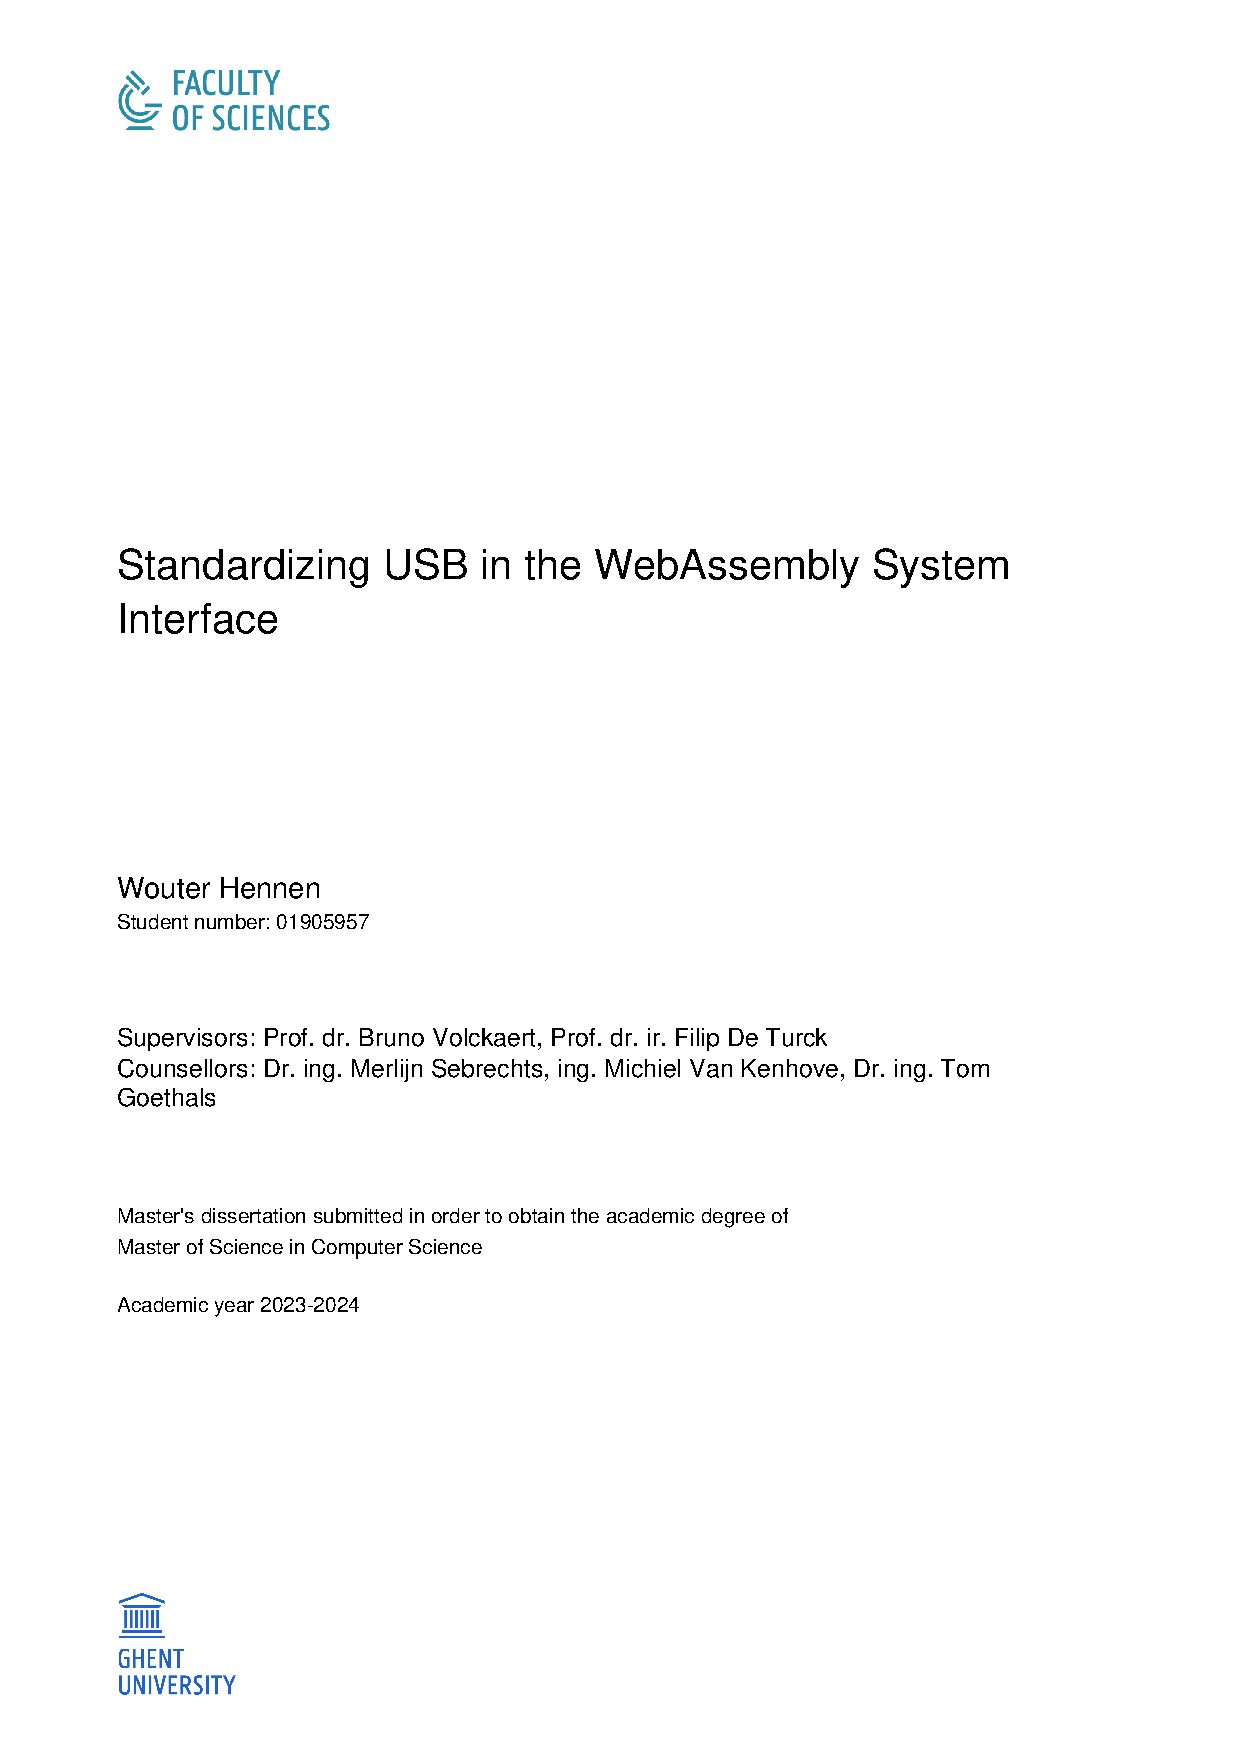
\includepdf{cover-sheet.pdf}

\chapter*{Acknowledgements}
I would like to thank my counsellors Dr. ing. Merlijn Sebrechts and ing. Michiel Van Kenhove for their help, commitment, feedback and time to make this thesis possible.

I would also like to thank my supervisors, Prof. dr. Bruno Volckaert and Prof. dr. ir. Filip De Turck.

Additionally, I would also like to thank my collegue Warre Dujardin for the collaboration on the proposal.

I would like to thank the WASI community for the creation of WIT, the available tooling and support.
\chapter*{Disclaimer regarding the master's thesis}

This master's thesis is part of an examination. Any comments made by the evaluation committee during the oral presentation of the master's thesis were not incorporated into this text.
\chapter*{Abstract}
\chaptermark{Abstract}
\addcontentsline{toc}{chapter}{Abstract}  

Updating software of \acrfull{IoT} devices is currently difficult. Having a longer lifespan than the average gadget, and oftentimes having special hardware and compilers that requires a lot of maintenance, most \acrshort{IoT} devices lose software support too soon \cite{wasi_iot}.
\acrfull{Wasm}, once made to run compiled code in a lightweight virtual machine in the browser, is trying to tackle this problem by expanding its support outside the browser. Because of its near-native performance, security, compactness and language interoperability, \acrshort{Wasm} is gaining popularity for its use on edge devices \cite{wasi_iot}. However, \acrshort{Wasm} lacks a proper interface to use outside the browser. To tackle this issue the \acrfull{WASI} was introduced, with the goal to provide a universal \acrshort{API} for all supported platforms and languages. \acrshort{WASI} is still in development and currently lacks an \acrshort{API} for using USB devices. The goal of this thesis is to research and develop an \acrshort{USB} \acrshort{API} for \acrshort{WASI}.

As part of the development is creating a proposal to extend the standard, where the interface of the \acrshort{API} is laid out and other matter, such as platform support, is further discussed. As part of this thesis, an initial proposal has been created \cite{wasi_usb}. The proposal has advanced to Phase 1 of the proposal process \cite{proposal_phases} and progress is being made to progress to Phase 2. The proposal contains a \acrshort{WIT} interface which supports enumerating devices, reading descriptors, connecting, reading and writing to devices and getting device connection updates. After doing research on existing similar solutions, such as WebUSB \cite{WebUSB} and \cite{LibUSB}, the proposal has taken inspiration from LibUSB. This makes it easier for developers to port existing applications to \acrshort{Wasm} as both LibUSB and \acrshort{WASI} \acrshort{USB} have similar interfaces. Some parts have been made different deliberately, for example the way file handles work. This way, the \acrshort{API} is easier to reason about. As \acrshort{Wasm} is sandboxed by default, access control is provided so programs do not have access to all devices by default. It is up to the user to specify which devices a program can access.

A reference implementation for the \acrshort{API} is provided \cite{wasi_usb} and extends the Wasmtime \cite{wasmtime_website} runtime to provide support for the \acrshort{USB} \acrshort{API}.

The implementation has been evaluated in three ways. First, a functional evaluation was made, testing the functionality of the API. In this evaluation, a guest module will observe connection events for a specific game controller, connect to the game controller, read out its state and control its rumble motors, confirming that the most important parts of the \acrshort{API} work.

Afterwards, the implementation has been evaluated for latency and memory usage. This is done by creating a \acrshort{USB} mass storage device driver by using the \acrshort{WASI} \acrshort{USB} \acrshort{API}. The file tree of a \acrshort{USB} drive can be read out and the file contents can be read. Comparing this against a native implementation shows on average a 4.2\% increase in latency, which is a good result. Memory usage using the \acrshort{WASI} \acrshort{API} is significantly higher, with the program using approx. 70\% more memory during heavy workloads, compared to native. This is likely caused by the way the memory model works in the Component Model, requiring the use of copying of data between components.

The \acrshort{WASI} \acrshort{USB} \acrshort{API} still has a long way to go before it is production ready, but the example programs in this thesis show the possibilities of the \acrshort{API} and demonstrate how the \acrshort{API} can be used in real-world use cases.
% How to add the extended abstract:
%
% You should write the extended abstract as a separate overleaf project. Then compile it there, download the PDF, and upload it to this project.
%
% Use the "IEEE conference proceedings template" to create the extended abstract project. 
% https://www.overleaf.com/latex/templates/ieee-conference-template/grfzhhncsfqn
%
% Then download the final PDF, upload it to the root of this project, and point the statement below to the correct file.
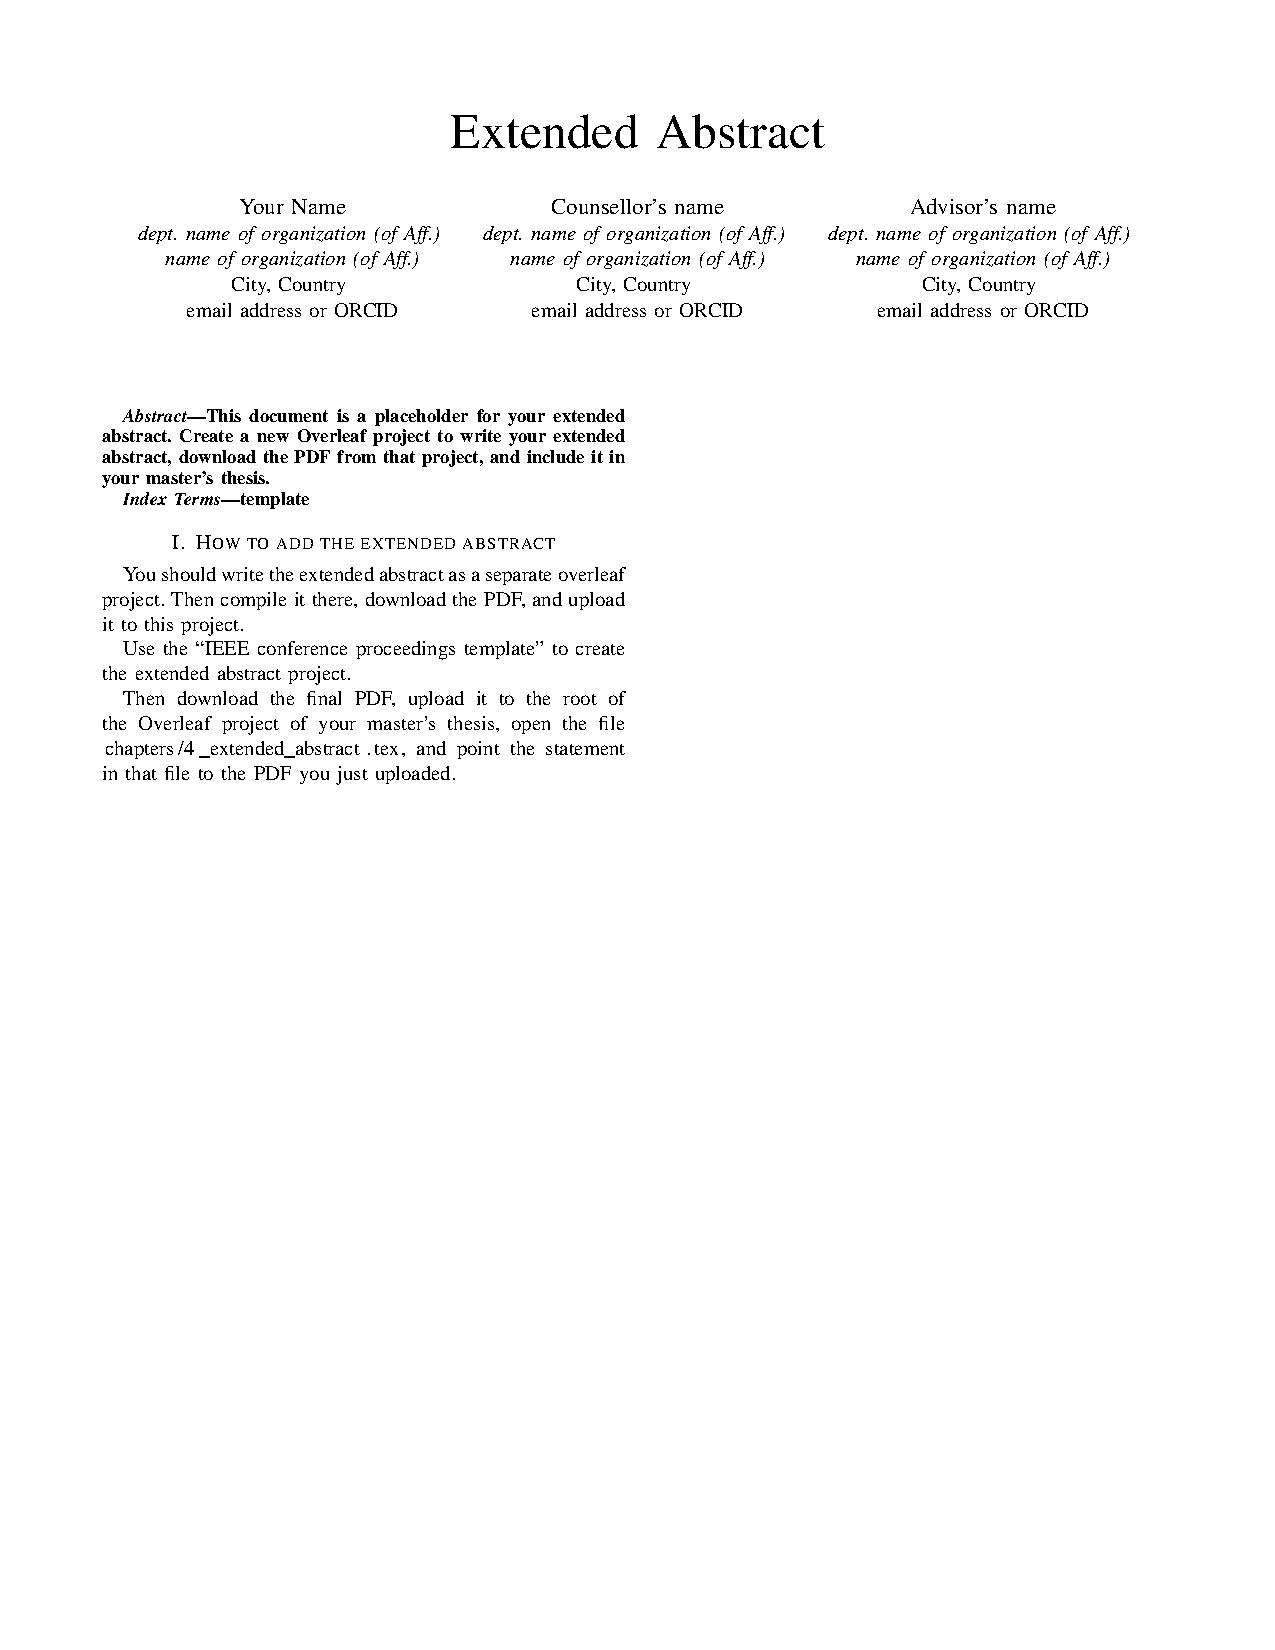
\includepdf[pages={-}]{extended-abstract.pdf}


\tableofcontents\newpage
\listoffigures\newpage
\listoftables\newpage
%%%%%%%%%%%%%%%%%%%%%%%%%%%%%%%%%%%%%%%%%%%%%%%%%%%%%%%%%%%%%%%
%                                                             %
% Note: To add or remove acronyms, modify `personal_data.tex` %
%                                                             %
%%%%%%%%%%%%%%%%%%%%%%%%%%%%%%%%%%%%%%%%%%%%%%%%%%%%%%%%%%%%%%%

\printnoidxglossary[type=\acronymtype, title={List of Acronyms}]
% \printglossary[type=\acronymtype, title={List of Acronyms}] % English

\glsaddallunused[\acronymtype]                              % make sure all unused acronyms are in list

\setlist[description]{style=standard} % reset list settings back to default

% \listoflistings\newpage

%
% Include the main chapters of the thesis below
% Note: it's best to avoid spaces in filenames as Latex might complain about them.
%
\mainmatter
\pagestyle{fancy} % Use header
\chapter{Introduction}
\label{chap:intro}

% In today's world, hyperscale cloud providers, such as Microsoft Azure and Amazon Web Services, are used extensively. These companies provide serverless functions, which run for short bursts and close immediately afterwards. In order to do this efficiently, the sandbox in which the code is executed should be able to quickly spin up, so the cold start problem can be minimized. Existing services like Docker and K8S are mostly used for this, but are not ideal: while being more performant than full blown operating systems, there cold boot is still problematic. A new standard, the WebAssembly System Interface (WASI), has been created which should greatly mitigate this problem.
% 
% \acrfull{Wasm} originally started as a way for browsers to execute code written in a language other than Javascript. It allows code from any supported programming language to be compiled to machine instructions for a virtual CPU, and for these instructions to be efficiently executed in the browser sandbox. This has proven to be successful and has opened numerous possibilities for web apps that weren't possible before. A great example of this is the new Google Earth website, which uses WebAssembly underneath, which allows for performant rendering of the Earth.
% 
% This model of running code on a lightweight virtual CPU seen interest outside of the browser, mainly for servers, low power devices (IOT), and so on. There, the WebAssembly System Interface could replace Docker, and provide performance improvements, power and storage savings.
% 
% WASI is currently still in development, and has a long way to go to get stable. One of the problems WASI is currently facing is the lack of APIs available to interface with the system. One of the APIs that is currently missing is the one to interact with USB devices. Having such an API would be useful for servers, cars, IOT devices, etc. The goal of this master's thesis is to create an USB proposal for expanding the WASI, and eventually add support for USB to WASI. With access control, users can decide which devices a program running in WASM can access.


% V2 TEKST

Updating software of \acrfull{IoT} devices is currently difficult. As the devices are home appliances, they are often used for longer periods of time, compared to other tech such as smartphones. As a consequence, these devices need longer software support. In reality, a lot of devices stop getting updates after a few years, making them vulnerable to cyberattacks. When an \acrshort{IoT} device gets hacked, it can be used as part of a botnet, or worse, send sensitive info (such as a video feed) to the attacker. There are multiple causes to why this software support period is short: no standardized updating mechanisms, special hardware and compilers, etc. \cite{wasi_iot}

In Web browsers, \acrfull{Wasm} acts as a generalized layer between the native browser API and a programming language. This model can also be applied outside the browser context and can solve some of the problems of native code. However, in order to do so, some changes are needed. As \acrshort{Wasm} is primarily targeted towards browser applications, it only provides libraries to do those things, for example accessing the DOM. No low-level libraries exist for controlling hardware devices, which would be required for \acrshort{IoT} devices. To solve this, a new specification was created: the \acrfull{WASI}

\acrshort{WASI} is a group of API specifications that can be used with software compiled to \acrshort{Wasm}. These APIs provide a standardized interface for any programming language that can compile to \acrshort{Wasm}. Because the APIs act as a layer between the native APIs and the application, access control can be applied to control what an application can access. To provide APIs that feel natural in any language, a new interface description language was born: \acrfull{WIT}. For each programming language, bindings can be created that expose a generalized API.

With \acrshort{WASI}, standardized APIs can be created that can be used to talk and control hardware. As the APIs are not device specific anymore and no compiling to specific architectures is needed anymore, updating software for \acrshort{IoT} devices has become a lot easier.

\section*{Problem Statement}

The \acrshort{WASI} standard is still in development and currently lacks an API to interact with USB devices. Having an API for USB devices is crucial for \acrshort{IoT} devices as a lot of hardware, such as cameras, will oftentimes communicate over USB.

\section*{Goal}

The goal of this master's thesis is to research and propose a new USB API for \acrshort{WASI}. Special attention will be given to access control, portability and performance.

\section*{Research Questions}

\begin{itemize}

\item What aspects of the USB interface can benefit of access control?

\item In what way can a WASI API be created that makes porting code easy?

\item What is the performance impact of this API compared to native code?

\end{itemize}

\chapter{USB Foundations}
\label{chap:rel_work}
In the early days of computers, various connectors existed for computers to communicate with external devices. A few examples of such connectors are the PS/2 port (Primarily used for Mouse / Keyboard) or the Parallel port (Often used for printers). These connectors have varying sizes, shapes and limitations and cannot be used for all devices. Therefore, computers needed to have all these ports, requiring lots of space. To address these issues, the USB connector was introduced. Years later, the interface has become the de-facto standard for wired device communication. Over the years, USB has evolved with multiple revisions. These revisions focus on key aspects of the interface, such as transfer speeds, power delivery and added functionality. The USB connector has also undergone revisions, making it smaller and reversible, so it is usable on a larger variety of devices.

In this thesis, the focus is on the software side of the USB standard. Therefore, the hardware will not be considered further.

\section{Transferring Data via USB}

This section introduces the internals of the USB protocol. For more information, take a look at \href{https://www.beyondlogic.org/usbnutshell/usb1.shtml}{USB in a NutShell} \footnote{https://www.beyondlogic.org/usbnutshell/usb1.shtml}.
\subsection{Pipes}
Data is transferred through pipes. A pipe is a connection from the host controller to the endpoint. Not all pipes are the same: they differ in the bandwidth they support, which transfer types are supported, in which direction data can flow, and their packet and buffer size. Pipes can generally be split up into two kinds.

\subsubsection{Streaming Pipes}
A Streaming Pipe is a one-way communication channel for the host or guest device to send any kind of data to the other end. This pipe is controlled by either the host of or guest device, and data is sent in a sequential way. The isochronous, interrupt and bulk transfer types will use this pipe to send data.

\subsubsection{Message Pipes}
A Message Pipe is a bidirectional communication channel. This pipe allows both the host and guest device to send commands in either direction on the same pipe. All message pipes are controlled by the host device. Only one transfer type supports this pipe: the control transfer type.

\subsection{Transfer Types}
\label{section:transfer_types}
The USB standard defines four transfer types. Each transfer type serves a different purpose, being optimized for speed, latency, correctness or reliability.

\subsubsection{Interrupt Transfer}
Interrupt transfers are most used for devices that transfer small amounts of data frequently. They have a bounded latency and are therefore suited for devices that require low latency and low bandwidth. Interrupt transfers can be initiated by both the host and guest device. The sent data will be queued by the sender, until the receiver polls the device.

Examples of devices that often use interrupt transfers are mice and keyboards.

\subsubsection{Isochronous Transfer}
Isochronous transfers are used for real-time data streaming. They provide a guaranteed data rate, but do not guarantee a correct transfer of data, and data can be lost. This makes the transfer type not suitable for situations where data integrity is important.

An example use case where isochronous data transfer is often used is streaming audio or video.

\subsubsection{Bulk Transfer}
Bulk transfers are suited for transferring large amounts of data where timing is not an issue, but data integrity is. No guarantee on timing is made, but guaranteed correct delivery is.

An example use case for bulk transfers is sending files to devices.

\subsubsection{Control Transfer}
Control transfers are used for configuration, command and status operations between the host and guest device. Control transfers operate on the Message pipe and has setup, data and handshake stages. The handshakes guarantee correct delivery, but will lead to a slower transfer speed. Therefore, control transfers are not used to transfer a lot of data, but rather for device initialization and control.

The Control transfer type can be seen as a TCP connection but for USB devices.

\subsection{Descriptors}

Descriptors are used numerous times throughout the USB specification. They define a standardized way to provide information about a part of the specification.

Details of each descriptor can be found in the appendix \ref{appendix:descriptors}.

\begin{figure}[h]
  \centering
  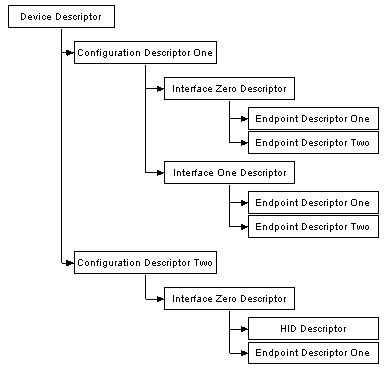
\includegraphics[width=0.5\textwidth]{images/descriptor_tree.png}
  \caption{Descriptor Tree of a USB device. This tree contains all useful metadata to communicate with the device.}
  \label{fig:descriptor_tree}
  \cite{USB_in_a_NutShell}
\end{figure}

\subsubsection{Device Descriptors}

Each USB device has a device descriptor which contains general information about the device, such as its device and vendor ID, which protocols it supports, its serial number, how much configurations it has, and more. This descriptor is essential, as it allows a program to find specific devices or kind of devices, so the right device can be chosen to communicate to.

\subsubsection{Configuration Descriptors}

The configuration descriptor provides information about a configuration of a USB device. A configuration describes the power usage of a device. For example, a device can have a configuration where it is self powered, and a configuration where it requires extra power from the host. Each configuration can have different combinations of interfaces and endpoints.

When a USB device is connected to a host, the host will examine the configuration descriptors and select the one required by the program.

\subsubsection{Interface Descriptors}

The interface descriptor provides information such as the interface number, the alternate setting number (if multiple settings are available for the interface), the number of endpoints associated with the interface, etc.

\subsubsection{Endpoint Descriptors}

Endpoints are the communication channels through which data is transmitted between the host device and the USB device.

The endpoint descriptor provides information such as the endpoint address, transfer speed, transfer type (see Section \ref{section:transfer_types}), etc.

Each endpoint can have any transfer type, except for endpoint zero. The zero endpoint is assumed to be a control endpoint, and will have a control transfer type. Endpoint zero will be used to communicate with the device to get its descriptors.

\section{Existing Solutions}

\subsection{libusb}
\label{section:libusb}
libusb \cite{LibUSB} is a versatile open-source library that offers platform-independent access to USB devices. Essentially, it is a thin wrapper around the system-provided USB APIs, providing a universal API. libusb is a C library and works on native hardware. It also works completely in user-mode, meaning no special privileges are required to communicate with USB devices. This makes it a very popular library to control USB devices, as it removes most issues that would occur when trying to support multiple platforms. It is also version-agnostic, so it will work with each USB protocol (1.0 - 4.0) \footnote{https://github.com/libusb/libusb/wiki/FAQ\#does-libusb-support-usb-3031324}.

As libusb makes creating cross-platform USB programs easy, it is used by most other technologies in this chapter, such as WebUSB (\ref{section:WebUSB}) and our own implementation (See Chapter \ref{chapter:implementation}).

\subsection{WebUSB}
\label{section:WebUSB}

WebUSB \cite{WebUSB} is a library to work with USB devices in browsers.

The WebUSB specification allows webpages to control non-standard USB devices. Browsers already provide easy APIs for common USB devices, such as mice, keyboards, cameras and microphones. However, accessing devices that do not follow these common USB use cases were not supported in the browser. In 2017, the WebUSB specification was created to provide a new API that allows this.

WebUSB has been proven useful in a lot of cases. For example, it has been used to control Arduino devices and upload new programs to these devices. Another kind of use case is to easily upgrade devices through USB, without the requirement to install special software. 

For example, after discontinuing its game streaming service Stadia, Google provided a firmware update for its Stadia controllers to enable bluetooth support \cite{stadia_bluetooth_mode} \cite{stadia_bluetooth_mode_explanation}. This update could be installed by connecting the controller to the computer and following the steps on the website. No additional software needed to be installed, making it very user-friendly.

WebUSB is not part of the web standards and is currently only supported in Chromium-based browsers. WebUSB only provides a limited Javascript API and is an abstraction over the raw USB interface, making it less useful for \acrshort{IoT} devices.

WebUSB can currently be used by \acrshort{Wasm} applications in the browser through the Javascript interface. However, this solution is far from ideal: there is additional overhead from using Javascript. Javascript is an interpreted language with dynamic and weak types. These capabilities make it harder to make a performant type-safe API. Furthermore, the API provides an abstraction over the USB specification and doesn't expose some parts of it.
\chapter{WebAssembly {\&} WebAssembly System Interface}
This chapter gives insight in what \acrfull{Wasm} is and how it works, alongside additional insight in how the \acrfull{WASI} works and how it is progressing.

\section{\acrshort{Wasm}}

When the web was born, the only supported programming language supported on the web was Javascript. As a relatively simple and portable language this did suffice. Over the years the web has become more complex and has become the center of the personal computer. However, its supported technologies did not grow at the same expansion pace. Javascript is still the only supported language and hampers the further expansion of the web. New technologies have been created to fix this issue, but none have succeeded. 
In order to be a viable Javascript alternative, a new model needs to be safe, fast, portable and compact. \acrshort{Wasm} is the first new technology to check all these four boxes. \cite{bringing_the_web_up_to_speed}

\subsection{Safe}
Wasm is intended to run in various environments, with some executing Wasm code from unknown sources. The web is a prime example of such a case. In these cases, it is required that the code runs in a sandbox, so that it cannot access all resources of the device. This way, malicious code can only do harm in the sandbox, and not the entire device.

Additionally, a Wasm program is often build in multiple modules. A Wasm module can be seen as an island of code, which imports and exports functions. Each module has its own stack, memory, types and more. This means that each module is isolated and cannot affect other modules, increasing the security of the model. Additionally, Wasm makes use of a linear memory model (Figure \ref{fig:wasm_high_level}). Each module gets its own range, and can only access that part of the memory.

\subsection{Portable}
\acrfull{Wasm} works as a compilation target for programming languages. Languages can compile to Wasm, just like they would for e.g. x86.
To compile to Wasm, the source code is first compiled to an intermediate representation, such as the LLVM IR. This is universal and also happens when compiling to other architectures. This part of the compilation process, called the frontend, stays the same. The backend of the compilation process, where the code gets translated into machine instructions, differs per instruction set. In the backend of the compiler the code will get compiled to the Wasm instruction set and output Wasm bytecode. This binary can get executed by a Wasm runtime. (Figure \ref{fig:wasm_compiler_frontend}) The bytecode is platform-agnostic, so it can run on any hardware and operating system that has a Wasm runtime. This makes Wasm portable.

This general idea works great for compiled languages, such as C, Rust or Swift. However, for interpreted languages such as Python, the model will work different. On native instruction sets, interpreted languages are read at runtime by their interpreter, which is often written in C. To make this work in Wasm, the interpreter can be compiled to Wasm and can interpret the language source code, just like it would happen on a native machine.

\subsection{Compact}
To achieve a small program, which is often critical for quickly loading websites, Wasm acts as a stack machine instead of a register-based machine. In register-based machines, registers are used to make calculations. On stack machines, argument values and operands are pushed on the stack, and result values are popped from the stack (Figure \ref{fig:wasm_high_level}). \cite{bringing_the_web_up_to_speed} By not having the need for registers, the binary size can be made smaller \cite{stack_vs_register_machine}. Another advantage of this method is that the amount of available registers can vary on different platforms. This is not an issue with stack machines.

\begin{figure}[h]
  \centering
  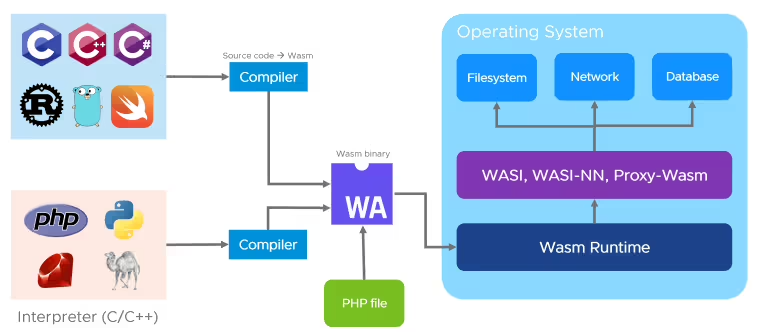
\includegraphics[width=1\textwidth]{images/wasm_compiler.png}
  \caption{Source code gets compiled to the Wasm architecture. The Wasm runtime executes the Wasm bytecode. \cite{docker_without_containers}}
  \label{fig:wasm_compiler_frontend}
\end{figure}

\begin{figure}[h]
  \centering
  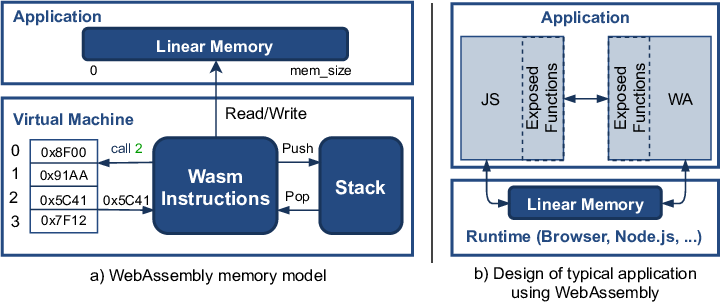
\includegraphics[width=1\textwidth]{images/WebAssembly-high-level-architecture.png}
  \caption{Wasm internals \cite{wasm_vulnerabilities}}
  \label{fig:wasm_high_level}
\end{figure}

\section{\acrshort{WASI}}

When writing code that compiles to Wasm, there is a need for system interfaces. These are required to do useful stuff, such as getting access to files. In the browser, WebAssembly applications can use Javascript as a system interface. However, outside the browser, there is no such predefined system interface. To solve this problem the \acrfull{WASI} was created. \acrshort{WASI} is a set of portable APIs, similar to APIs you would find in an operating system.

\subsection{The Component Model}

\subsection{\acrshort{WIT}}

\subsection{Milestones}


\chapter{Architecture}
\label{chap:evaluation}

In dit hoofdstuk ...

\section{Sectie titel}
\label{sec:scalable_faafo}

Vul aan...

\chapter{Implementation}
\label{chapter:implementation}
This chapter dives deeper into the internals of the API. First, an overview will be given of how a typical series of calls works under the hood. Next, the runtime implementation will be discussed. At last, using the \acrshort{API} in a guest component will be explained.

The repository containing the code can be found \href{https://github.com/Wouter01/USB_WASI}{here} \footnote{https://github.com/Wouter01/USB\_WASI}.

\section{Overview}

Figure \ref{fig:implementation_overview} shows the series of calls that happen in a typical, albeit small, use case of the API. The program functionality is the following:
\begin{enumerate}
\item Get all devices.
\item Find the device needed.
\item Open the device and select the right configuration / interface.
\item Read data from the device.
\item Close the device.
\end{enumerate}

Under the hood a lot more is happening, which can be seen in the figure. Most calls can be forwarded to LibUSB, which will handle OS-specific behaviour. Some steps, like opening a device, require some extra work in the runtime.

On the left side of the figure are the function calls to LibUSB shown. On the right side are the calls shown from and to the \acrshort{Wasm} guest. The function names are of the format \texttt{wit\_interface.\{function\_name\_in\_interface\}}.

\begin{figure}[h]
  \centering
  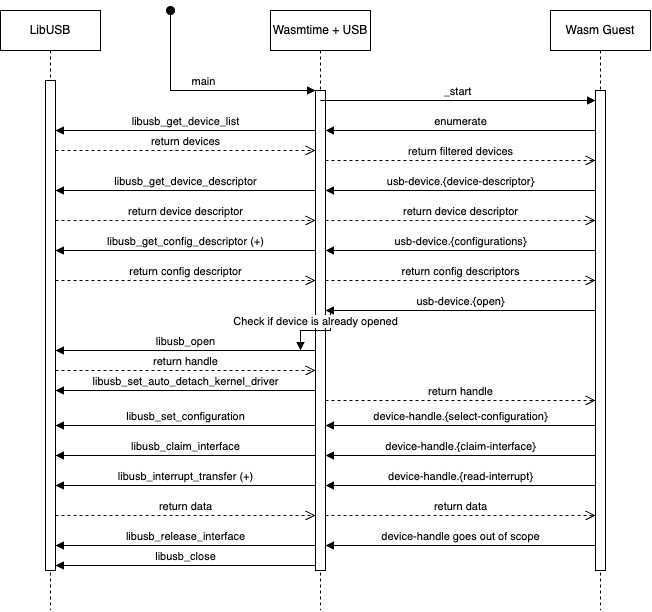
\includegraphics[width=0.8\textwidth]{images/sequentiediagram.png}
  \caption{Typical series of events sent between Wasm module - Wasmtime - LibUSB.}
  \label{fig:implementation_overview}
\end{figure}


\section{Runtime Implementation}
One of the requirements when proposing a new \acrshort{WASI} \acrshort{API} is to have multiple runtime implementations of that \acrshort{API}. This is required in order to advance to phase 3 of a proposal. The \acrshort{USB} \acrshort{WASI} proposal is still at phase 1. However, having a working implementation of the developing \acrshort{API} makes it easier to test out ideas and spot issues quickly. It also is useful to determine the viablity of the \acrshort{API}. Therefore, a runtime implementation has been created before the proposal process has started.

When creating the \acrshort{PoC} implementation, a \acrshort{Wasm} runtime must be chosen which will be extended by the \acrshort{API}. There are numerous \acrshort{Wasm} runtimes available, such as Wasmtime \cite{wasmtime_website}, Wasmer \cite{wasmer} or WasmKit \cite{wasmkit}. Wasmtime was chosen for implementing the \acrshort{PoC}, as it has support for the Component Model and it is developed by the Bytecode Alliance, the organization behind \acrshort{WASI}.

\subsection{Choosing the programming language}
The implementation is written in Rust \cite{rust_lang}, a system-level programming langauge which focuses on performance and safety. Rust's performance is similar to that of C, but its design eliminates entire classes of memory related bugs. Rust was an easy choice, as it has great support for \acrshort{Wasm} and \acrshort{WASI}, and Wasmtime is also written in it.

\subsection{Interfacing with LibUSB}
As told in section \ref{section:libusb}, LibUSB will be used to communicate with operating-specific APIs to communicate with USB devices. LibUSB is written in C. It is possible to interface with C in Rust. To make things easier, the Rusb \cite{rusb} package is used, which acts as a thin Rust wrapper around the LibUSB C API.

\subsection{Interfacing with Wasmtime}
Wasmtime can be used in two ways: 
\begin{itemize}
\item Using the default Wasmtime runtime through the command line. A compiled \acrshort{Wasm} module can be passed as an argument:
\begin{minted}{bash}
$ wasmtime hello.wasm
Hello, world!
\end{minted}
\item Embedding the Wasmtime runtime in another app. The Bytecode Alliance provides packages in multiple languages, such as Rust or Go, to do this \cite{wasmtime_website}. This is the method used for creating the \acrshort{PoC} and is discussed further below.
\end{itemize}

The \acrshort{PoC} runtime embeds the Wasmtime runtime. The method of running is also similar: a compiled \acrshort{Wasm} module is passed as a command line argument.

Code snippet \ref{code:main} shows the main function of the runtime. First, the arguments are parsed, which contain the path to the component to run and identifiers of USB devices which are visible to components using the \acrshort{USB} \acrshort{API}. Next, the component gets instantiated (see code snippet \ref{code:start_component}) and an allowlist of devices is created. Finally, the component gets started.

The main function is annotated with \texttt{\#[tokio::main]}, meaning that the asynchronous Tokio runtime \cite{tokio} will be used. Tokio is an asynchronous runtime for Rust, and is not related to the Wasmtime runtime. The use of an asynchronous runtime is done for two reasons:
\begin{itemize}
\item The Wasmtime configuration in the runtime has enabled async support. At the time of writing, this isn't a really useful addition \cite{wasmtime_async_config}. However, this will become more useful once \acrshort{WASI} preview 3 lands, which will add proper async support to the \acrshort{WIT} language. Enabling async support now partially prepares for this upcoming feature.

\item The runtime receives updates when USB devices are connected and disconnected. This feature runs blocking functions which run on a separate thread. Tokio makes this easy to do.\\
\end{itemize}


\begin{code}
\begin{minted}[tabsize=4]{rust}
#[tokio::main]
async fn main() -> Result<()> {
	let parsed = UsbDemoAppParser::parse();
	let mut app = UsbDemoApp::new(parsed.component_path)?;

	let allowed_devices = if parsed.usb_use_denylist {
		AllowedUSBDevices::Denied(parsed.usb_devices)
	} else {
		AllowedUSBDevices::Allowed(parsed.usb_devices)
	};

	app.start(allowed_devices).await?
		.map_err(|_| anyhow!("Failed to run component."))
}
\end{minted}
\caption{The main function will start running the guest component.}
\label{code:main}
\end{code}

Code snippet \ref{code:start_component} shows how the passed in component will get instantiated. The \texttt{main} function first calls the \texttt{new} function. This function creates some necessary objects: 
\begin{itemize}
\item \texttt{Config}: The configuration used when creating a new \texttt{Engine}.
\item \texttt{Engine}: An engine manages and compiles Wasm modules.
\item \texttt{Linker}: A linker is used to link components. Each component defines imports and exports. The linker is used to resolve these imports and exports, and throw errors if the required imports cannot be resolved.
\item \texttt{Component}: Used to represent a \acrshort{WASI} component.
\item \texttt{Store}: \say{A Store is a collection of WebAssembly instances and host-defined state.
All WebAssembly instances and items will be attached to and refer to a Store. For example instances, functions, globals, and tables are all attached to a Store. Instances are created by instantiating a Module within a Store.} \cite{wasmtime_store}
\end{itemize}

Next, the built-in components are added to the linker. \texttt{wasmtime\_wasi::add\_to\_linker\_async} adds all the standard Wasmtime components to the linker, such as \texttt{wasi:cli/stdout}. \texttt{Imports::add\_to\_linker} links the USB \acrshort{WIT} interface. Finally, the command component is loaded in and compiled.

The \texttt{start} function creates a new \texttt{Store} object. This object is associated with the earlier created engine, and contains the memory for an instance of \texttt{USBHostWasiView}. Finally, an instance of the guest component is created. We assume that the component is a \texttt{Command} (\ref{section:component_kinds}) and therefore exposes a \texttt{main} function. The \texttt{main} function, in \acrshort{WASI} terms also known as the \texttt{\_start} function, gets called.\\

\begin{code}
\begin{minted}[tabsize=4, breaklines]{rust}
struct UsbDemoApp {
	engine: Engine,
	linker: Linker<USBHostWasiView>,
	component: Component
}

impl UsbDemoApp {
	fn new(component: PathBuf) -> Result<Self> {
		let mut config = Config::default();
		config.wasm_component_model(true);
		config.async_support(true);

		let engine = Engine::new(&config)?;
		let mut linker = Linker::new(&engine);

		wasmtime_wasi::add_to_linker_async(&mut linker)?;
		Imports::add_to_linker(&mut linker, |view| view)?;
		
		let component = Component::from_file(&engine, component)?;

		Ok(Self {
			engine,
			linker,
			component
		})
	}

	async fn start(&mut self, allowed_devices: AllowedUSBDevices) -> anyhow::Result<Result<(), ()>> {
		let data = USBHostWasiView::new(allowed_devices)?;
		let mut store = Store::new(&self.engine, data);
	
		let (command, _) = Command::instantiate_async(&mut store, &self.component, &self.linker).await?;
	
		command.wasi_cli_run().call_run(store).await
	}
}
\end{minted} 
\caption{Code for extending the Wasmtime runtime.}
\label{code:start_component}
\end{code}

\subsection{Conforming to the \acrshort{WIT} interface}
The runtime must conform to the \acrshort{WIT} interface described in section \ref{section:usb_proposal}. This part of the code \textit{receives} requests from guest components using the interface. The communication between the host and a component happens through the canonical ABI. As discussed in section \ref{section:thecomponentmodel}, bindings can be used to ease the translation from and to the canonical ABI format. Wasmtime offers the \texttt{bindgen} macro \cite{wasmtime_component_bindgen} to generate such bindings in Rust.

The usage of the \texttt{bindgen} macro is shown in code snippet \ref{code:wit_bindgen}.
This macro will generate Rust types and traits that represent their \acrshort{WIT} counterparts. The host must conform to all these traits. Otherwise, adding the \acrshort{USB} \acrshort{WIT} interface to the linker will be disallowed.

The \texttt{with} map shown in code snippet \ref{code:wit_bindgen} is used to point the \texttt{bindgen} tool to the Rust types we want to use to represent the \texttt{usb-device} and \texttt{device-handle} resources. The \texttt{bindgen} macro will use these types in the generated traits.\\

\begin{code}
\begin{minted}[tabsize=4, breaklines]{rust}
pub mod bindings {
	wasmtime::component::bindgen!({
		world: "component:usb/imports",
		async: true,
		with: {
			"component:usb/usb/usb-device": crate::device::usbdevice::USBDevice,
			"component:usb/usb/device-handle": crate::device::devicehandle::DeviceHandle,
		},
		path: "../WIT/wit"
	});
}
\end{minted} 
\caption{Bindings are generated by using the Wasmtime \texttt{bindgen} macro.}
\label{code:wit_bindgen}
\end{code}

Code snippet \ref{code:conforming_example} shows an example usage of the generated bindings:
\begin{itemize}
\item \textbf{\texttt{USBHostWasiView}} is the type that implements the \acrshort{USB} \acrshort{WIT} interface. An instance of this type is passed to the linker to represent the \acrshort{USB} interface. The type checker verifies that \texttt{USBHostWasiView} conforms to all the required traits.
\item \textbf{\texttt{HostDeviceHandle}} is the trait generated by the bindings. It contains functions which \texttt{USBHostWasiView} needs to conform to.
\item \textbf{\texttt{Resource<DeviceHandle>}} is a reference to an \texttt{DeviceHandle} instance. 
\end{itemize}

\texttt{DeviceHandle} has a handle that is used to call LibUSB functions. In this example, the \texttt{claim\_interface} function will call the equivalent LibUSB function and return its result.\\

\begin{code}
\begin{minted}[tabsize=4, breaklines]{rust}
#[async_trait]
impl HostDeviceHandle for USBHostWasiView {
	async fn claim_interface(&mut self, handle: Resource<DeviceHandle>, interface: u8) -> Result<Result<(), DeviceHandleError>> {
		let result = self.table()
			.get_mut(&handle)?
			.handle
			.claim_interface(interface)
			.map_err(|e| e.into());
	
		Ok(result)
	}
}

pub struct DeviceHandle {
	pub handle: rusb::DeviceHandle<rusb::Context>
}
\end{minted} 
\caption{An example of using generated bindings. An implementation for \texttt{claim-interface} is provided.}
\label{code:conforming_example}
\end{code}

\subsection{Conforming to constraints}
Section \ref{section:capability_based_security} and \ref{section:usage_in_multiple_components} mention important constraints regarding the correct implementation of the API. The implementation conforms to the following constraints.

\paragraph{Capability-based security}
As seen in code snippet \ref{code:main}, an allowlist gets created, containing a series of device IDs. A device is identified by the pair \texttt{vendor\_id:product\_id}. These can be passed in as arguments when running the program. An optional flag \texttt{--usb-use-denylist} can be given so the program uses a denylist instead of an allowlist.

\begin{verbatim}
cargo run -- --usb-devices 18d1:9400,18d1:9401 guest-component.wasm
\end{verbatim}

Table \ref{table:allowlist} shows the four configurations that are possible. The functions \texttt{usb-device.\{enumerate\}} and \texttt{events.\{update\}} will use this configuration to filter out devices that should not be visible.

\begin{table}[h!]
\centering
\begin{tabular}{|c|c|c|}
\hline
& \textbf{Allowlist} & \textbf{Denylist} \\
\hline
\textbf{Devices Specified} & specified devices allowed & all but specified allowed \\
\hline
\textbf{No devices specified} & no device allowed & all allowed \\
\hline
\end{tabular}
\caption{Device Access Control.}
\label{table:allowlist}
\end{table}

\paragraph{Usage in multiple components} Exclusive access to devices is guaranteed by keeping track of the device handles. Only one \texttt{device-handle} instance may exist for each \acrshort{USB} device. \texttt{USBHostWastView} stores a set of device addresses for devices with an active \texttt{device-handle}. It does not keep track of which component uses which device. When an \texttt{device-handle} gets dropped, the device address is removed from the set and becomes available again. When a component tries opening an already-opened device, an error will be thrown. 

\subsection{Platform limitations}
\label{section:platform_limitations}
The current host implementation works on Linux, macOS and Windows. However, some features work slightly different on some platforms:

\begin{itemize}
\item macOS: 
\begin{itemize}
\item Using devices for which the kernel provides drivers is disallowed, unless the program has elevated privileges, for example using \texttt{sudo} \cite{libusb_macos_limitations}.
\end{itemize}

\item Windows:
\begin{itemize}
\item LibUSB hotplug support is currently missing for Windows. This feature is used in the implementation to get device connection events. Recent activity shows that this might come soon \cite{libusb_hotplug_support}.
\item HID keyboards and mice cannot be accessed using the native HID driver as Windows reserves exclusive access to them \cite{libusb_windows_limitations}. 
\end{itemize}
\end{itemize}

\section{Usage in guest components}
This section demonstrates how a \acrshort{WASI} component can use the \acrshort{USB} \acrshort{API}. Parts of the code used for the program in section \ref{section:functional_evaluation} will be explained.

\subsection{Defining a \acrshort{WIT} interface}
The guest component is required to also provide a \acrshort{WIT} interface, shown in code snippet \ref{code:guest_world}. The interface contains a single \texttt{root} world, describing the imports and exports required by the component. The guest component explained here is a Command component (\ref{section:component_kinds}), and therefore does not provide any exports. In order to use the \acrshort{USB} \acrshort{API}, it will import all the interfaces of the \acrshort{USB} component.\\

\begin{code}
\begin{minted}[tabsize=4, breaklines]{rust}
package component:usb-component-wasi-stadia;

world root {
	import component:usb/types@0.2.0;
	import component:usb/usb@0.2.0;
	import component:usb/events@0.2.0;
	import component:usb/descriptors@0.2.0;
}
\end{minted} 
\caption{The \acrshort{WIT} world for the guest component.}
\label{code:guest_world}
\end{code}

\subsection{Creating a \acrshort{Wasm} module}
The code written for the guest component must be compiled to a .wasm file. Doing this can be time consuming, as multiple steps are required:

\begin{enumerate}
\item Create bindings.
\item Build a \acrshort{Wasm} module.
\item Create a new \acrshort{WASI} component and apply the adapter for \acrshort{WASI} preview 2.
\end{enumerate}

In order to ease this process, the Cargo-component tool \cite{cargo_component} was created. By running
\begin{verbatim}
cargo component build
\end{verbatim}
the tool will interpret the \acrshort{WIT} interface, generate bindings for Rust code, and produce a compiled \acrshort{Wasm} module. The guest component makes use of this tool to produce a \acrshort{Wasm} module with ease.

\subsection{Calling the \acrshort{USB} \acrshort{API}}
Now that the \acrshort{WIT} interface is defined and bindings are created, calling the USB API is straightforward. Code snippet \ref{code:calling_usb_api} shows the \texttt{main} function of the guest component. This function will start listening to connection events, and calls the \texttt{component:usb/events{update}} function to get these events. Next, it will match the event using the \texttt{component:usb/events{device-connection-event}} variant. As can be seen in the code snippet, these \acrshort{WASI} types are translated to Rust types and can be imported into the file. Then, they can be used like regular Rust code. \\

\begin{code}
\begin{minted}[tabsize=4, breaklines]{rust}
use crate::bindings::component::usb::{
	usb::UsbDevice, 
	events::DeviceConnectionEvent
};

#[tokio::main(flavor = "current_thread")]
async fn main() -> anyhow::Result<()> {
	loop {
		match update() {
			DeviceConnectionEvent::Pending => sleep(Duration::from_secs(1)).await,
			DeviceConnectionEvent::Connected(device) if device.is_stadia_device() => {
				// Found stadia controller
				... // Handle
			},
			DeviceConnectionEvent::Disconnected(device) if device.is_stadia_device() => {
				// Stadia controller is removed
				... // Handle
			},
			_ => continue
		}
	}
}
\end{minted} 
\caption{The \acrshort{WIT} world for the guest component.}
\label{code:calling_usb_api}
\end{code}


\chapter{Proposal}

\chapter{Evaluation}

\section{Functional Evaluation}
\label{section:functional_evaluation}
When developing the API, it is useful to already have guest code utilizing the API to quickly iterate. The following proof of concept is one of the guest programs created to test the API. It touches on all the parts of the API: getting device updates and receiving and sending data through the USB interface. As it is a proof of concept, it does not test the performance of the API.

The general idea of the program is to control a game controller. The program is started and observes the connected devices. Once a controller is connected that is recognized by the program, the program will connect to the controller. The state of all the controls of the device will be read, and input updates will be print out. To test sending data over the USB interface, the program will send commands to the controller to activate the rumble motors \footnote{Rumble motors are used to vibrate the controller}.

\subsection{Test Setup}
The code will call the event-related API to start watching for USB devices. It will get events when devices are connected or disconnected. As WASI does not support asynchronous code yet, a form of polling is used to get device connection events. The guest code uses a single-threaded asynchronous runtime, which will often yield to get new device connection events. This way, a multi-threaded real app can be simulated.

\begin{enumerate}
\item Each time a device connection event happens, the device product and vendor ID are checked to see if they match the predefined controller product and vendor ID. A Google Stadia controller is used to test this code, so the IDs of this controller type are used.

\item Make a connection and open a device handle if the device IDs match.

\item Select the correct configuration and interface. Input devices, like controllers or mice, send their data over the Interrupt transfer type, because the data sent is small and time-sensitive. Knowing this information, the interfaces can be requested and filtered to select the correct interface. macOS is used to run this example which offers default drivers for controllers, so elevated privileges are needed to detach the kernel drivers. Otherwise, the program cannot claim the interrupt interface.

\item Read the controller state from the interrupt interface, such as which buttons are pressed, what the position of the joysticks is, etc. An array of bytes is received, and by observing changes to this array when pressing a button, the byte layout can be decoded.

\item Print out the controller state. A sample output is showed in Code snippet \ref{code:wasi_controller_sample_output}.

\item Make the controller vibrate. This happens when the program state reports that one of the shoulder buttons has registered pressure. The state of the shoulder buttons is mapped to intensity of the rumble motors. This data is sent over the interrupt interface. When the controller receives the data it starts vibrating.

\item When a device disconnection event with matching IDs happens, the program will stop reading the controller state, close the device handle, and wait for a new connection.


\end{enumerate}

% Each time a device connection event happens, the device product and vendor ID are checked to see if they match the predefined controller product and vendor ID. A Google Stadia controller is used to test this code, so the IDs of this controller type are used. If the IDs match, a connection is made to the device by opening a device handle. When a device disconnection event with matching IDs happens, the program will stop reading the controller state, and wait for a new connection.
% 
% Next, the program will try reading the controller state. This way, it knows about the positions of buttons, joysticks, triggers, etc. In order to do this, the correct interface and endpoint must be chosen. Input devices, like controllers or mice, send their data over the Interrupt transfer type, because the data sent is small and time-sensitive. Knowing this information, the interfaces can be requested and filtered to select the correct interface. In order to send information over the interface, it must first be claimed by the program. Some operating systems will attach to the interfaces by default. The host code of the API will automatically disconnect kernel attachments when claiming an interface. However, different operating systems can have different behavior in this part. For example, macOS, where the example program was ran on, does not allow detaching kernel interfaces by default for certain device classes, such as controllers. This is problematic, as we cannot interact in any way with the device this way. Elevated privileges (\texttt{sudo}) were required to get the program working. While being annoying, this was also a useful discovery, as this issue can be added to the proposal, so the standard can adjust to this.
% 
% Once the interface is claimed, device state can be requested by reading the interrupt state with the correct endpoint address. An array of bytes will be received, and by observing what changes when pressing a button, the byte layout can be decoded. A sample controller state output is showed in Code snippet \ref{code:wasi_controller_sample_output}.

\begin{code}
\begin{verbatim}

dpad: ,
buttons: assistant_button|l2_button|r2_button,
left stick: x: 128 y: 128,
right stick: x: 128 y: 128,
l2: 255,
r2: 172
\end{verbatim}
\caption{Output after reading controller state.}
\label{code:wasi_controller_sample_output}
\end{code}

\subsection{Results}
This program has been tested with a Google Stadia controller. When pressing one or multiple buttons, the correct state is printed out. When pressing one or both of the shoulder buttons, the controller starts to vibrate.



\section{Hardware \& Software Configuration}

Tests were performed to evaluate the performance of the API. In these tests, test programs are created which run in WASI, as a native program or, when available, on Wasm in the browser. Table \ref{table:test_hardware} shows the hardware configurations of the devices used to do these tests. Table \ref{table:software_environment} shows the software environment in which the tests were performed.

\begin{table}[H]
\[
\begin{array}{|l|l|l|l|l|l|}
\hline
\textbf{Device} & \textbf{Name} & \textbf{SoC/Microcontroller} & \textbf{RAM} & \textbf{Storage} & \textbf{USB Version} \\
\hline
\text{Host} & \text{Apple Macbook Air (2020)} & \text{Apple M1 (8-core CPU, 7-core GPU)} & \text{8GB} & \text{256GB SSD} & \text{4.0} \\

\hline
\text{Guest} & \text{Arduino Micro} & \text{Atmel ATmega32U4} & \text{2,5KB} & \text{32KB Flash} & \text{2.1} \\

\hline
\text{Guest} & \text{Samsung T5 Portable SSD} & \text{} & \text{} & \text{500GB SSD} & \text{3.1 Gen 2} \\
\hline
\end{array}
\]
\caption{The hardware used for testing the performance of the API.}
\label{table:test_hardware}
\end{table}

\begin{table}[h]
\centering
\begin{tabular}{|l|l|}
\hline
\textbf{Operating System} & macOS 14.5 \\ \hline
\textbf{Wasm Runtime} & Wasmtime 20.0.2 \\ \hline
\textbf{USB Library} & libusb 1.0.27, Rusb 0.9.4 \\ \hline
\textbf{Rust Version} & rustc 1.78.0 \\ \hline
\end{tabular}
\caption{Software Environment.}
\label{table:software_environment}
\end{table}


\section{Latency Evaluation}

One of the advantages of \acrshort{Wasm} should be that it offers near-native speed. Therefore, it is interesting to test if running a program in Wasm brings any performance overhead compared to a native program. For an USB API, this can best be tested by measuring the latency when sending or receiving data. It can be problematic if the overhead is large, as data exchange through USB happens by receiving or sending data in small chunks. Each of these chunks has to pass through the Wasm bridge and has its own overhead.

\subsection{Receiving data from Arduino}

\subsubsection{Test Setup}
A program has been written with LibUSB (Native) and WASI USB (Wasm). Each program will do the following steps:

\begin{enumerate}
\item Enumerate the USB devices.
\item Find the Arduino board, based on its product and vendor id.
\item Open the device and claim the Bulk interface.
\item Send the \acrfull{DTR} signal to the Arduino. This signal is sent to the Arduino to acknowledge that the host device is ready to receive data. Once the Arduino has received this signal, its setup phase is completed and it will start sending data.
\item \textit{Warm up } the interface by throwing away the first batch of readings. By doing this, initial latency is removed from the measurements.
\item Read data from the Bulk interface, while measuring how long this operation takes. The arduino sends data in batches in 64 bytes, and the program will read them a million times. The program will throw away the read results, so only the transfer of the data is measured. In total, 64MB is received by the host.
\item Write durations to file.
\end{enumerate}

\subsubsection{Results}
Figure \ref{fig:arduino_reading_latency_boxplot} shows a boxplot of the latencies of both programs. After a million measurements for each program, the median duration is exactly the same, 377μs. The average of the native program is marginally lower, being 0,2\% faster than the \acrshort{WASI} program. The whiskers and IQR of the \acrshort{WASI} program are slightly smaller, meaning a more consistent result. However, the differences in results are too small to conclude any noticeable overhead.

\begin{figure}[H]
  \centering
  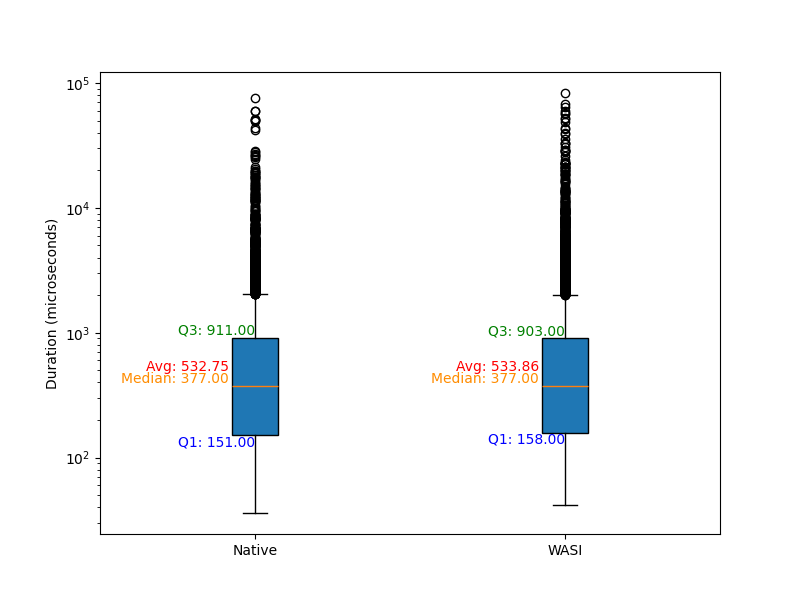
\includegraphics[width=1\textwidth]{images/arduino_latency_boxplot.png}
  \caption{Latency of reading data from Arduino using read-bulk.}
  \label{fig:arduino_reading_latency_boxplot}
\end{figure}


Figure \ref{fig:arduino_reading_latency_boxplot} also contains outliers, marked by the black circles. Some of the outliers are very large. Therefore, the results are shown on a logarithmic scale. These outliers are likely caused by transmission errors when receiving data from the Arduino. The \textit{Bulk} interface is used, providing data integrity but no timing guarantees. Consequently, data loss will be prevented, but will introduce high latencies as observed here. Table \ref{table:latency_comparison} shows more information about the outliers. As the percentage of outliers is very small and occur in equal quantities in both cases, they have been excluded from further figures to improve the clarity of the graphs.

\begin{table}[h]
\centering
\begin{tabular}{|l|c|c|}
\hline
 & \textbf{Native} & \textbf{WASI} \\ \hline
\textbf{Largest Outlier (μs)} & 75618 & 83052 \\ \hline
\textbf{Amount of Outliers (\textgreater 2000)} & 747 & 1058 \\ \hline
\textbf{Percentage of Total} & 0.07\% & 0.10\% \\ \hline
\end{tabular}
\caption{Comparison of Latency Outliers between Native and WASI.}
\label{table:latency_comparison}
\end{table}



Figure \ref{fig:arduino_reading_latency} shows a \acrfull{KDE} for the measurements of the native and \acrshort{WASI} implementation.
Both graphs will show peaks around the 150μs and 910μs marks. This is an interesting result, as one would expect one uniform distribution instead of two. The first peak is trivial to explain: the Arduino is an USB 2.0 device, also known as a High-speed USB device. A High-speed USB device will send frames at a fixed interval of 125μs. Therefore, we will receive new data approx. every 125μs. An extra 25μs are introduced because of processing delays. 

The second peak is more nuanced. Table \ref{table:arduino_output} shows a snippet of the measured latencies. For both Native and WASI code, the latencies will oscillate between both peaks. Based on these results, this peak is likely caused by the small buffer size in the Arduino. The buffer is 64 bytes large, which is the same size as one packet. When the buffer is full, the program halts until the buffer has space again. On the host this is perceived as an extra delay when receiving the data.

\begin{figure}[H]
  \centering
  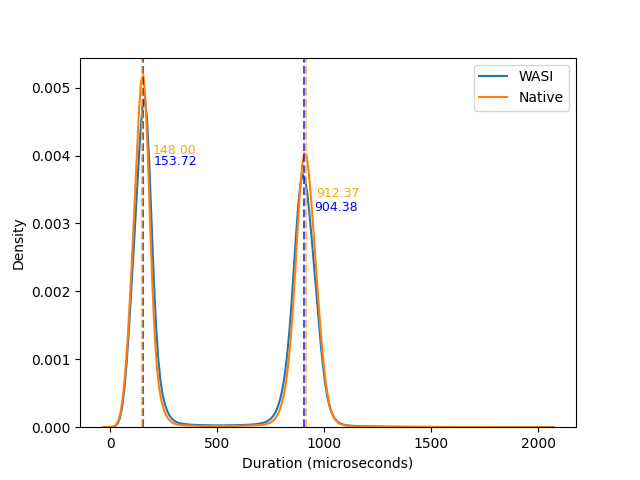
\includegraphics[width=1\textwidth]{images/reading_data_latency.png}
  \caption{Latency of reading data from Arduino using read-bulk.}
  \label{fig:arduino_reading_latency}
\end{figure}

\begin{table}[h!]
\centering
\begin{tabular}{|l|l|}
\hline
\textbf{Native (μs)} & \textbf{WASI (μs)} \\
\hline
801 & 918 \\
\hline
150 & 163 \\
\hline
885 & 931 \\
\hline
132 & 241 \\
\hline
903 & 799 \\
\hline
110 & 197 \\
\hline
938 & 820 \\
\hline
104 & 77 \\
\hline
962 & 1003 \\
\hline
108 & 97 \\
\hline
\end{tabular}
\caption{Snippet of measured latencies. The latencies oscillate between a long latency and a short latency.}
\label{table:arduino_output}
\end{table}

Based on the results, we can conclude that there are no measurable differences between the native and \acrshort{WASI} program. However, this is mainly caused by the delay of the USB protocol. This delay vastly outweighs the delays caused by overhead of the Wasm runtime, making the Wasm overhead negligible.

However, it is possible that the delay of the USB protocol is smaller on devices more powerful than an Arduino or with a more modern USB version. With these configurations, it can be possible a small overhead for Wasm becomes visible.

\subsection{Reading files from Mass Storage device}
\label{section:mass_storage_latency}

In order to confirm that WASI does not add noticeable latency, another benchmark is performed, which reads the contents of an USB Mass Storage device. The advantage of this benchmark compared to the Arduino benchmark is that it better represents real-world usage, instead of being a synthetic benchmark.

\subsubsection{Test Setup}
A program has been written which enumerates the file tree of a USB device and reads the contents of each file in the file tree. A Samsung T5 External SSD is used to perform these tests. The device is connected with a cable that supports a transfer speed up to 5Gb/s and is formatted with the \acrshort{MBR} partition map and the \acrshort{exFAT} file system. There are 10 files stored on the device, most of which are a few KBs in size. One file has a size of 679MB. In total, 680MB is stored on the device.

The program contains a working but incomplete implementation for the \acrshort{USB} Mass Storage Bulk-Only transport specification. Further information about the specification and implementation details can be found in the specification documents \cite{usb_specification_boot} \cite{usb_specification_bulk}. The code exposes an interface where one can \textit{seek} to a specific address and \textit{read} the contents from there up until a specified length.

\paragraph{\acrshort{USB} \acrshort{API} Usage}
As the name of the specification suggests, communication with the device happens on the interfaces with the \textit{Bulk} transfer type. Some exceptions, such as the \texttt{reset} command, will use the \textit{Control} transfer type on interface zero.

\paragraph{Reading drive contents}
The \acrshort{USB} Mass Storage implementation acts as the base layer to communicate with the device. However, further abstraction is required. USB Mass Storage devices can still differ in numerous ways:

\begin{itemize}
\item Partition Map: A disk is usually split up in multiple partitions. A partition map contains information about those partitions. It is located in the first sector (sector 0) of the device. Popular partition maps are the \acrfull{MBR} and the \acrfull{GPT}. The test device has a \acrfull{MBR} partition map. The Rust package \textit{mbrman} \cite{mbrman} is used to read the \acrshort{MBR} and obtain the start and end addresses of the partition which contains the file system.

\item File System: The file system organizes files and their metadata in a defined format. There exist a lot of file systems, but the most popular for Mass Storage devices are \acrfull{FAT32}, \acrfull{exFAT} and \acrfull{NTFS}. The test device uses the \acrshort{exFAT} file system. The test program uses the \textit{exfat} \cite{exfat_package} Rust package to interpret the \acrshort{exFAT} partition.
\end{itemize}

Both \textit{mbrman} and \textit{exfat} use the Mass Storage implementation to read data at addresses. Code snippet \ref{code:implementation_mass_storage} shows how the Mass Storage implementation is used to read the files.

\begin{code}
\begin{minted}[breaklines, tabsize=4]{rust}

fn main() {
    // Open the Mass Storage device.
    let mut device = MassStorageDevice::new()?;
    let block_length = device.capacity.block_length;

    // Read the MBR to get information about the device partitions.
    let mbr = mbrman::MBR::read_from(device, block_length)?;

    // Select the first used partition.
    let data_partition = mbr.iter().find(|p| p.1.is_used())
        .ok_or(anyhow!("No used partition found"))?.1;

    // Apply a slice to the device stream, so only the selected partition is considered when reading.
    let slice_start = ...
    let slice_end = ...
    let slice = IoSlice::new(device, slice_start, slice_end)?;

    // Apply buffering to the stream to increase performance.
    let buffered_stream = BufReader::new(slice);
    
    // Open the exFAT file system.
    let filetree = ExFat::open(buffered_stream)?;

    // Recursively read the device tree.
    for item in filetree {
        read_item(item)?;
    }
}
\end{minted}
\caption{Code to read files and directories from the Mass Storage device.}
\label{code:implementation_mass_storage}
\end{code}

With a working implementation to read out the file tree, a benchmark can be performed. The benchmark enumerates the file tree and reads out the contents of each file, and reports each file size and name. The duration of this operation is logged. This is repeated 1000 times, so the file tree will be read out 1000 times. This is done for the program running in Wasmtime using the \acrshort{USB} \acrshort{API} and a native program using Rusb \cite{rusb}.

\subsubsection{Results}

Figure \ref{fig:mass_storage_latency_naive} shows a boxplot with the results of reading the file tree and file contents of the device. With a lower average and median, the \acrshort{WASI} program seems to outperform the native program. The average execution time of the native program is 12\% slower than the \acrshort{WASI} program, the median execution time is 18\% slower. This is odd, as one would expect the native version to be faster.

However, there is an explanation for this behaviour. The program will read out the entire contents of the disk, which is in total around 3GB. Each file will be loaded into memory and immediately discarded. The disk contains a few files with a size of over 500MB. Loading these files into memory becomes expensive due to the amount of \texttt{malloc}s that need to happen. Profiling the code shows more insights.

The code is compiled in debug mode so debug symbols are added to both programs, so we can interpret the system calls easier. This will lead to a significantly slower running program, especially for the \acrshort{WASI} program. This is not a problem as the profiling is only used to measure memory usage and not speed. The sample size is also lowered to 10 samples instead of 1000.

Figure \ref{fig:malloc_instruments} shows the total time spent on \texttt{malloc} for the native program. 25\% of the execution time was spent on allocating memory, which is a significant amount. Figure \ref{fig:malloc_wasi_instruments} shows that the \acrshort{WASI} program only spends 0,6\% of its execution time on \texttt{malloc} and therefore does not have this issue. This happens because of the way a \texttt{Store} works in Wasmtime: \say{A Store is intended to be a short-lived object in a program. No form of GC is implemented at this time so once an instance is created within a Store it will not be deallocated until the Store itself is dropped.} \cite{wasmtime_store}. Because no memory is freed, the already-allocated memory can be reused, avoiding extra \texttt{malloc} and \texttt{free} calls. A Wasmtime \texttt{Store} therefore can act as a memory pool, which can be significantly faster than using \texttt{malloc} \cite{memory_pool_wikipedia}.


\begin{figure}[H]
  \centering
  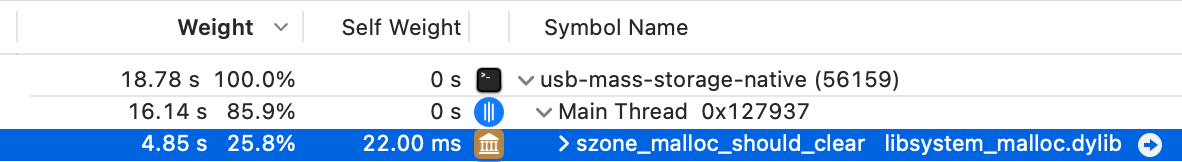
\includegraphics[width=1\textwidth]{images/malloc_screenshot.png}
  \caption{Approx. 25\% of the native program execution time is spent on \texttt{malloc}.}
  \label{fig:malloc_instruments}
\end{figure}

\begin{figure}[H]
  \centering
  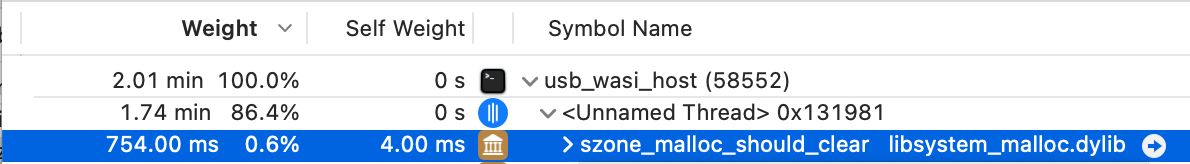
\includegraphics[width=1\textwidth]{images/malloc_wasi_screenshot.png}
  \caption{Approx. 0.6\% of the \acrshort{WASI} program execution time is spent on \texttt{malloc}.}
  \label{fig:malloc_wasi_instruments}
\end{figure}

\begin{figure}[H]
  \centering
  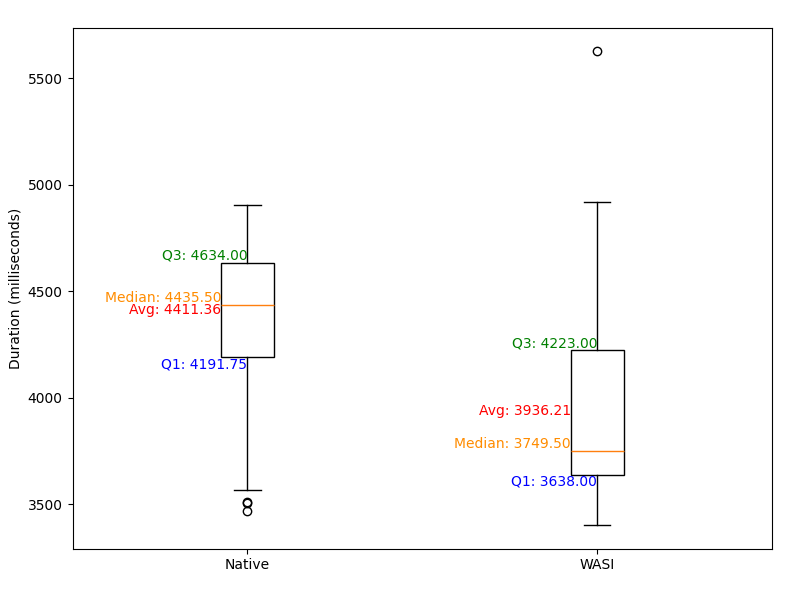
\includegraphics[width=1\textwidth]{images/mass_storage_1000_runs_naive.png}
  \caption{Latency of reading the file tree and contents. The \acrshort{WASI} results incorrectly report a better result due to differences in memory allocation between both programs. On average, the native program is 12\% slower.}
  \label{fig:mass_storage_latency_naive}
\end{figure}



\subsubsection{Improving results}

To make a better measurement at the latency of the \acrshort{USB} \acrshort{API}, the test has been modified. Instead of the test running multiple times in the guest code, the guest component runs multiple times. Each time, a new \texttt{Store} will be created. This will let the memory allocation behave similar to the native program.

Figure \ref{fig:mass_storage_latency_optimized} shows a boxplot with the new measurements. The measurements of the native program are the same as in Figure \ref{fig:mass_storage_latency_naive}. The average \acrshort{WASI} program execution time is 4,2\% slower than the average native program, and the median 4,3\% slower. The \acrshort{WASI} program also has more outliers, indicating that the performance of the \acrshort{WASI} program may be less consistent.

\subsubsection{Conclusion}
Based on these results, we can conclude that running the code using the \acrshort{WASI} \acrshort{USB} \acrshort{API} introduces a small amount of overhead. Caution must be exercised when benchmarking memory-intensive \acrshort{Wasm} programs to obtain accurate results.

\begin{figure}[H]
  \centering
  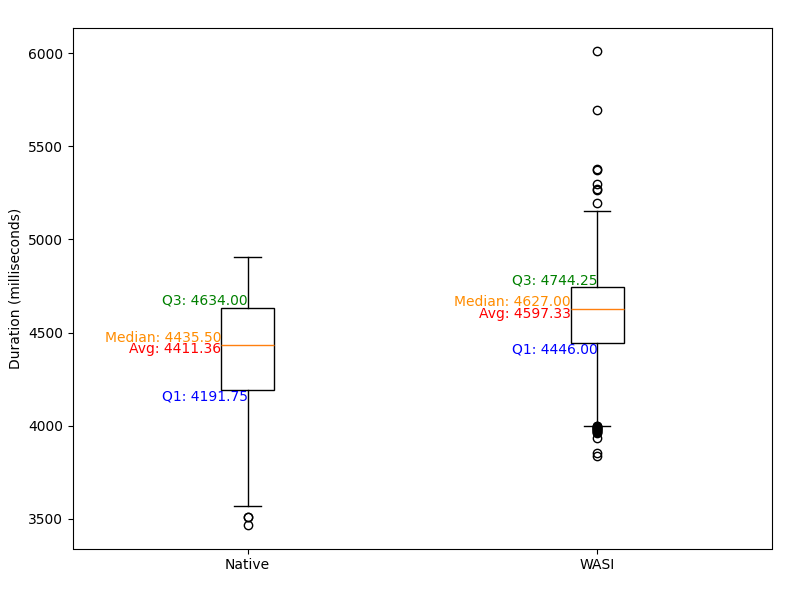
\includegraphics[width=1\textwidth]{images/mass_storage_1000_runs_optimized.png}
  \caption{Latency of reading the file tree and contents after changing the benchmark method. Both programs now use a similar memory allocation method leading to more accurate results. On average, the \acrshort{WASI} \acrshort{USB} implementation is approx. 4,2\% slower.}
  \label{fig:mass_storage_latency_optimized}
\end{figure}

\section{Memory Usage Evaluation}
In contrast to standard \acrshort{Wasm} modules, \acrshort{WASI} components have separate memory spaces. As a result, one component cannot read or write the memory of another component \cite{memory_model}. This improves the security of the Component Model and the interoperability between components, but can also add additional memory usage due to the need of copying memory. Therefore, it is interesting to see how much impact \acrshort{WASI} has on the memory usage of a typical program.

\subsection{Reading files from Mass Storage device}
\label{section:reading_files_memory}
The same test setup as \ref{section:mass_storage_latency} will be used to benchmark memory usage. Section \ref{section:mass_storage_latency} already discussed a performance issue caused by memory allocation. As this section is about the \textit{amount} of memory used, and not about the \textit{performance} of utilizing it, this problem won't be further discussed here.

\subsubsection{Test Setup}
\label{section:reading_files_memory_test_setup}
Some changes are made to the test setup described in \ref{section:mass_storage_latency}. Instead of logging the duration of reading the file tree, the amount of memory will be logged. Also, instead of running the benchmark 1000 times, it is now run once.

The method to measure the memory will differ slightly in both implementations. Using a profiler to measure the memory has given incorrect results when benchmarking the \acrshort{WASI} implementation. Therefore, no profiler is used for this benchmark. Instead, the memory size is checked numerous times during the execution of the program. This is done getting the \textit{real} memory size of the program every millisecond. For the \acrshort{WASI} program this is done in Wasmtime. A baseline memory usage is also measured for the \acrshort{WASI} program which gets loaded but does not do anything.

The program will also sleep 3 seconds before and after opening and closing the device, so the memory usage evolution can be better seen.

\subsubsection{Results} 

Figure \ref{fig:mass_storage_memory_comparison} shows the differences in memory usage for both programs. As both programs consume a lot of memory, the initial Wasmtime memory usage is neglected, as it does not have a large influence on the results. The influence of initial Wasmtime memory is discussed in section \ref{section:travering_file_tree_memory}.

After the initial 3 seconds of waiting time, both programs start traversing the file tree and reading the contents. It is clear that the \acrshort{WASI} program uses more memory and with more spikes. As memory is not shared, values are copied over from host to guest, increasing the memory usage. At its peak, it will use 1239MB, while the native program uses 718MB. This is 72,5\% more. This peak happens when reading in the largest file of 679MB. As the disk is mostly empty, data is stored contiguously on the disk. This improves reading performance and ensures a steady flow of data at the receiver's end. This is clearly visible in the graph for the native program, as its memory usage follows a linear function. The \acrshort{WASI} implementation contains more spikes. These spikes are likely caused by the copying of values, which rapidly allocates and deallocates memory.

After the contents have been read, memory usage will quickly drop for both programs. However, memory usage for the \acrshort{WASI} program will decrease slower than the native program. This mainly happens because of the memory-pool-like behavior of the \texttt{Store} \cite{wasmtime_store}, which will not deallocate memory. Memory used outside the \texttt{Store} will still get deallocated, which is why there is a memory decrease. Once the program ends the memory will get freed further.

\begin{figure}[H]
  \centering
  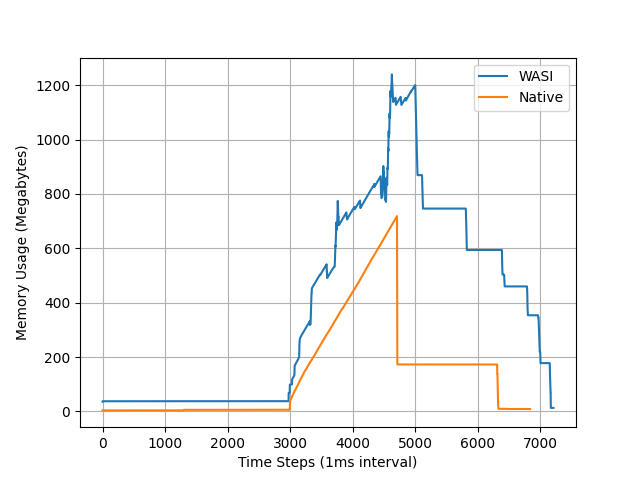
\includegraphics[width=1\textwidth]{images/mass_storage_comparison.png}
  \caption{Memory usage when traversing the file tree and reading the file contents. At the end of reading the largest file (678MB), the \acrshort{WASI} program will consume 72,5\% more memory than the native counterpart.}
  \label{fig:mass_storage_memory_comparison}
\end{figure}



\subsection{Traversing file tree from Mass Storage device}
\label{section:travering_file_tree_memory}
A less memory-intensive benchmark was also performed to check how \acrshort{WASI} memory usage would compare when using less memory. This benchmark uses the same test setup as \ref{section:reading_files_memory}, except that it will not read out the file contents. The file tree has also changed and now contains 11947 files, with a total size of 3,25GB.

\subsubsection{Results}

Figure \ref{fig:mass_storage_file_tree_comparison} shows the results of the benchmark. The graph contains the results of the total memory usage of both programs, and also contains the \acrshort{WASI} results without the initial memory occupied by Wasmtime. This is a useful metric, as a program utilizing the \acrshort{USB} \acrshort{API} can be part of a larger piece of code, where the initial memory overhead of Wasmtime gets \textit{distributed} between all components and can be neglected.

The first 3000 measurements show the memory usage from when the program is sleeping for 3 seconds, as described in \ref{section:reading_files_memory_test_setup}. The memory of both native and \acrshort{WASI} programs are similar, not accounting for the initial Wasmtime memory usage. Furthermore, the \acrshort{WASI} memory usage is slightly better at the start, but this is likely caused by applying the correction. Once the useful program code starts, memory will spike for both programs. However, the \acrshort{WASI} (corrected) program will approx. 63MB of memory, 69,8\% more than the native's 37,1 MB memory usage.

\begin{figure}[H]
  \centering
  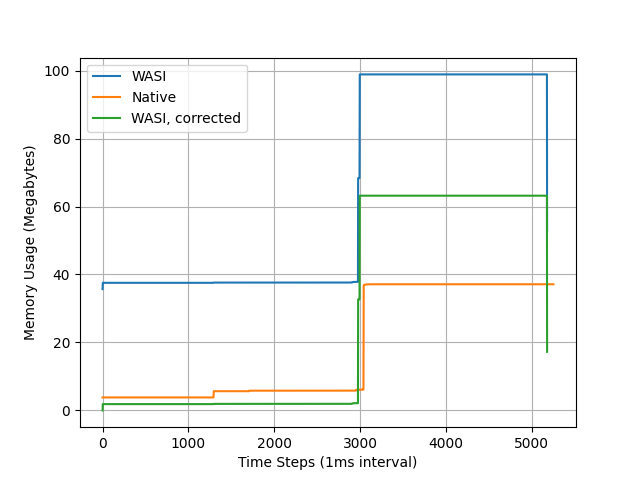
\includegraphics[width=1\textwidth]{images/mass_storage_memory_filetree_with_correction.png}
  \caption{Memory usage when traversing the file tree. The \acrshort{WASI} program consumes 69,8\% more memory than the native counterpart.}
  \label{fig:mass_storage_file_tree_comparison}
\end{figure}
\chapter{Conclusion}

The \acrfull{WASI} is rapidly progressing. While still in development, the initial vision of the people behind the Bytecode Alliance is coming to life and will hopefully get to a stable state in the coming years. This masters thesis has done research on the possibilities of utilizing \acrshort{USB} devices in \acrshort{WASI} and will hopefully make a positive impact on the eventual support of it. 

The proposal that was developed over the year, together with the initial working implementation in Wasmtime, has dug through most of the questions and issues that one would expect when developing such an \acrshort{API}. While the proposal still has a long way to go, it has laid out the fundamentals of the \acrshort{API} which can be expanded further upon.

One of the most prevalent questions was how access control, one of the prime features of \acrshort{WASI}, could be integrated in the \acrshort{API}. After trying out multiple possibilities, it was concluded that limiting access control on a device-level is deemed enough. The idea is also worked out in the implementation and functions as expected. The proposal also contains directions for adding access control to other parts of the interface, should this be needed.

Multiple \acrshort{API} designs were tested out, one leaning more to what libusb offers, while the other leaning more into WebUSB. After trying out both \acrshort{API}s and getting feedback from the community, an \acrshort{API} which closely follows libusb was chosen. This \acrshort{API} is more aligned with how \acrshort{USB} devices work internally. This also makes it easier for existing programs using libusb to port their code over to \acrshort{WASI} \acrshort{USB}.

Performance of the \acrshort{API} has been thoroughly tested and results are overall positive. \acrfull{Wasm} is fast enough to not have notable performance issues when using the \acrshort{USB} \acrshort{API}, especially when compared to the latency of communicating with an external device. However, due to the isolated memory of \acrshort{WASI} components, data sent from and to a device needs to be copied, bringing in memory overhead. This can become a problem for applications that use a lot of memory.


\chapter{Future Work}
Research done for this thesis has laid the groundwork for building a \acrshort{WASI} \acrshort{USB} \acrshort{API}. However, the proposal is still at phase 1 and has a long way to go before it can become stable. Further work will need to happen on testing, providing multiple runtime implementations, creating fully functional programs that utilize the \acrshort{API} and gaining further community feedback.

Also, the \acrshort{API} currently has some shortcomings that will need to be addressed in the future:

\begin{itemize}
\item The proposal currently ignores language support, but \acrshort{USB} devices can provide certain data, like device names, in multiple languages.
\item Windows hotplug support is currently missing, making the \texttt{events} interface of the proposal currently unavailable for Windows. As discussed in Section \ref{section:platform_limitations} this could be solved soon.
\end{itemize}
\renewcommand\bibname{Referenties}
\bibliography{referenties}

\begin{appendices}
\section*{Bijlage A}
\addcontentsline{toc}{section}{Bijlage A}  

Toelichting bijlage.



\newpage
\section*{Bijlage B}
\addcontentsline{toc}{section}{Bijlage B}  

Toelichting bijlage.

\end{appendices}


\pagestyle{numberless} 
\pagestyle{empty}
\begin{appendices}
\section*{Bijlage A}
\addcontentsline{toc}{section}{Bijlage A}  

Toelichting bijlage.



\newpage
\section*{Bijlage B}
\addcontentsline{toc}{section}{Bijlage B}  

Toelichting bijlage.

\end{appendices}


\end{document}
